\documentclass[11pt,a4paper]{article}

\usepackage[T1]{fontenc}
\usepackage[utf8]{inputenc}
\usepackage[brazil]{babel}
\usepackage{lmodern}
\usepackage[margin=2.5cm]{geometry}
\usepackage{booktabs}
\usepackage{tabularx}
\usepackage{amsmath,amssymb}
\usepackage{graphicx}
\usepackage{xcolor}
\usepackage{enumitem}
\usepackage{listings}
\usepackage{tikz}
\usetikzlibrary{arrows.meta,positioning,calc,fit,backgrounds}
\usepackage{titlesec}
\usepackage{caption}
\usepackage[hidelinks]{hyperref}

\definecolor{verde}{HTML}{2F7D4F}
\definecolor{azul}{HTML}{0B7AA8}
\definecolor{laranja}{HTML}{C05621}
\definecolor{cinza}{HTML}{5F6B62}
\definecolor{fundo}{HTML}{F4F6F3}

\titleformat{\section}{\Large\bfseries\color{verde}}{\thesection}{0.6em}{}
\titleformat{\subsection}{\large\bfseries}{\thesubsection}{0.6em}{}
\titleformat{\subsubsection}{\normalsize\bfseries}{\thesubsubsection}{0.6em}{}
\setlist{itemsep=2pt,topsep=4pt}
\captionsetup{font=small,labelfont=bf}

\lstset{
  basicstyle=\ttfamily\small,
  backgroundcolor=\color{fundo},
  frame=single, rulecolor=\color{fundo},
  breaklines=true, columns=fullflexible, keepspaces=true,
  showstringspaces=false, upquote=true,
  xleftmargin=4pt, xrightmargin=4pt, aboveskip=6pt, belowskip=6pt,
  literate={á}{{\'a}}1 {à}{{\`a}}1 {ã}{{\~a}}1 {â}{{\^a}}1 {é}{{\'e}}1 {ê}{{\^e}}1
           {í}{{\'i}}1 {ó}{{\'o}}1 {õ}{{\~o}}1 {ô}{{\^o}}1 {ú}{{\'u}}1 {ç}{{\c c}}1
           {Á}{{\'A}}1 {É}{{\'E}}1 {Ç}{{\c C}}1 {°}{{$^\circ$}}1 {×}{{$\times$}}1
}
\newcommand{\cod}[1]{\texttt{#1}}
\newcommand{\feito}{\textcolor{verde}{$\blacksquare$}}
\newcommand{\falta}{\textcolor{cinza}{$\square$}}

\title{\textbf{\Huge GAIA}\\[6pt]
\Large Monitoramento de plantas com câmera, sensores e IA\\[4pt]
\large Protótipo embarcado: nó de captura, servidor de inferência e documentação}

\author{Miguel Pereira \quad Thiago Almeida \quad Leticia Sabadini \quad Gabriel Borges\\[8pt]
\normalsize Multivix Serra\\
\normalsize \url{https://github.com/MrWlker/gaia-project}}
\date{Setembro de 2026}

\begin{document}
\maketitle
\thispagestyle{empty}

\begin{abstract}
\noindent
O GAIA é um protótipo embarcado de fenotipagem de plantas. Um nó de captura,
formado por um Raspberry Pi~3, uma câmera Intel RealSense D435 e sensores de
ambiente, fotografa o canteiro em intervalos e grava cada captura em disco antes de
enviá-la. Um servidor de inferência, num computador com GPU, encontra as plantas na
imagem, reconhece cada uma pela posição ao longo do tempo, estima o ambiente no
ponto de cada planta e classifica espécie, condição, agente, órgão e hidratação com
um modelo multi-cabeça sobre um tronco ConvNeXt-Base, que recebe também as leituras
de temperatura e umidade. Este documento descreve a arquitetura, a rede, o servidor,
o nó de captura, a preparação do Raspberry Pi e o caminho para construir outros
protótipos a partir do código. O código e esta documentação estão no repositório;
o modelo pré-treinado é publicado à parte, e o código de treino e os dados
acompanham o artigo.
\end{abstract}

\clearpage
\begin{figure}[t]
  \centering
  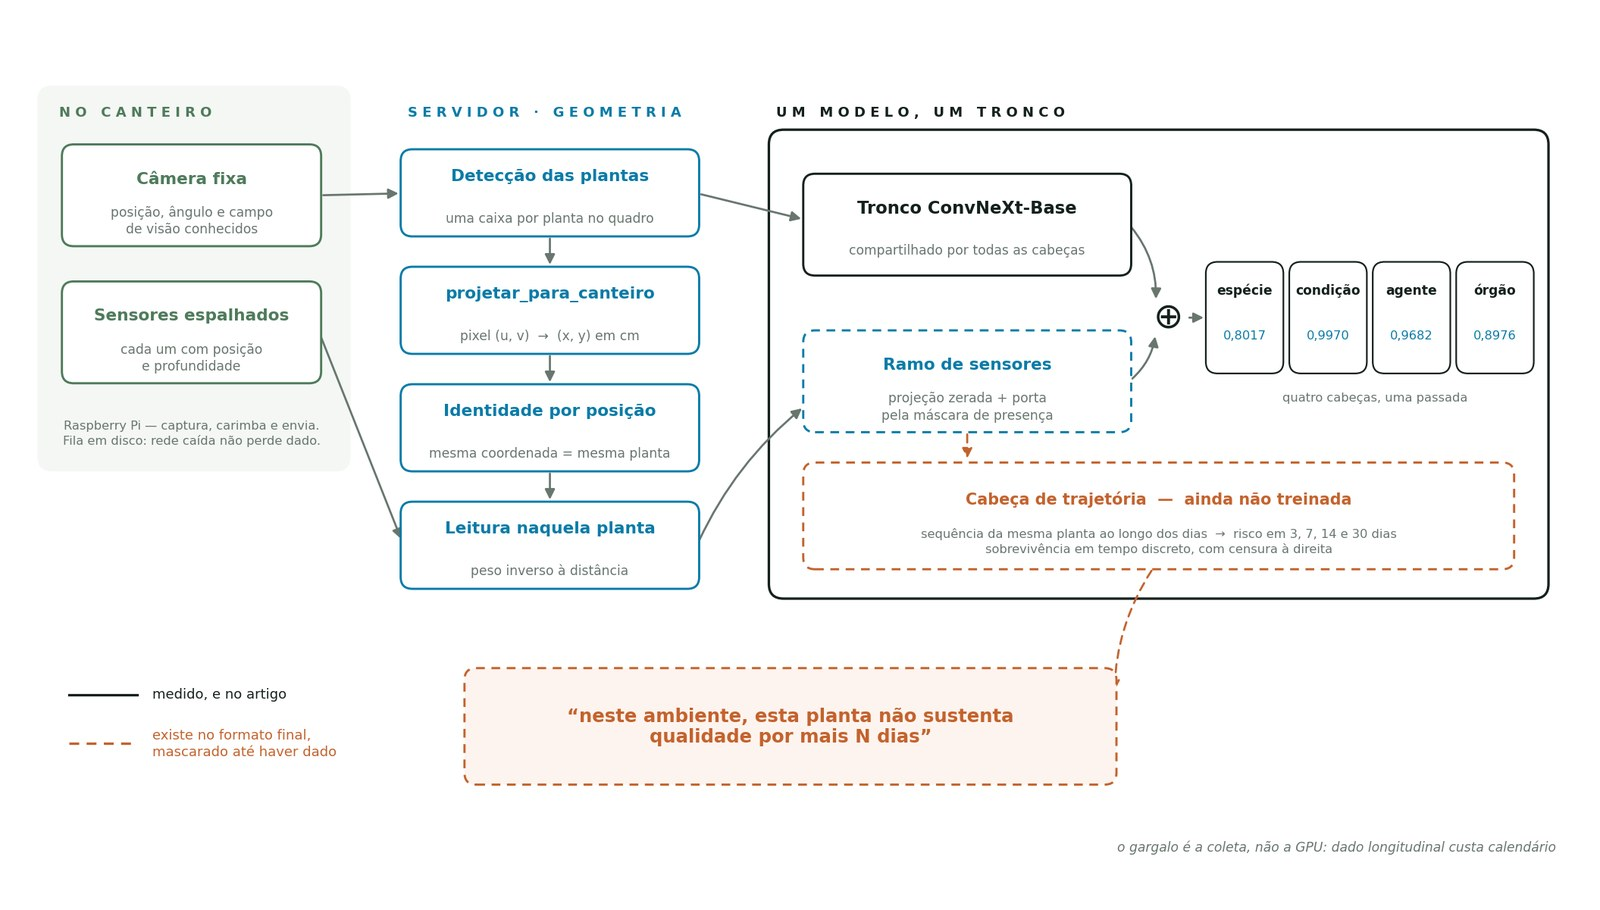
\includegraphics[width=\linewidth]{../figuras/arquitetura.jpg}
  \caption{Arquitetura do GAIA: o nó no canteiro, a geometria no servidor e o modelo
  com tronco compartilhado, ramo de sensores e cabeças por pergunta. Tracejado: parte
  que existe no formato final e aguarda dado.}
  \label{fig:arquitetura}
\end{figure}

\tableofcontents
\clearpage

% =====================================================================
\section{Visão geral}

\subsection{O problema}
Classificar uma foto de folha não basta. O objetivo do GAIA é acompanhar
\textbf{cada planta ao longo do tempo} --- a mesma planta hoje, amanhã e na semana
seguinte --- junto do ambiente em que ela vive, para no futuro prever a trajetória de
saúde dela. Isso impõe três decisões de projeto que aparecem em todo o código.

\paragraph{Identidade da planta pela posição.}
A câmera é fixa e a planta não anda. Cada detecção é projetada do pixel para uma
coordenada $(x, y)$ em centímetros no canteiro, e duas detecções a menos de 20~cm
uma da outra, em dias diferentes, são a mesma planta. Não há rede de rastreamento
nem cadastro manual. A origem das coordenadas é o controlador do canteiro; câmeras e
sensores são cadastrados pelo deslocamento até ele.

\paragraph{O sensor que vale é o mais próximo da planta.}
Com vários sensores espalhados, a leitura atribuída a cada planta é a interpolação
por inverso da distância no ponto dela, não a média do canteiro. Cada leitura é uma
linha por sensor por instante, porque uma coluna anônima ``solo1'' não sabe a que
pedaço do canteiro pertence.

\paragraph{Dado longitudinal não se refaz.}
Perder uma semana de captura custa uma semana de calendário. Por isso o nó grava
primeiro em disco e envia depois; se o servidor cai, a fila cresce e escoa quando ele
volta. Leitura que falha vira \emph{ausente}, nunca um valor inventado.

\subsection{Onde cada coisa roda}
O Raspberry Pi~3 tem 1~GB de RAM e um Cortex-A53 sem aceleração útil para
convolução; só o ConvNeXt pede centenas de megabytes de ativação a 384~px. Por isso
\textbf{nenhuma rede neural roda no Pi}: ele captura, carimba, guarda e envia. O
mesmo código do nó roda num PC, o que permite desenvolver a interface e a inferência
com a câmera no notebook antes de o Pi estar pronto.

\subsection{O que acontece numa captura}
\begin{enumerate}
  \item O nó pede à câmera o próximo quadro alinhado e grava na fila três arquivos: a
  cor (JPEG), a profundidade (PNG de 16~bits, em milímetros, alinhada à cor) e um JSON
  com as leituras e a intrínseca de fábrica da câmera.
  \item Envia ao servidor (\cod{POST /ingest}); se falhar, a captura fica na fila.
  \item O servidor encontra as regiões de vegetação e, para cada uma: projeta no
  canteiro, acha ou cria a planta, interpola os sensores ali, classifica o recorte e
  calcula o Grad-CAM da condição.
  \item Grava tudo e desenha a imagem anotada (caixas, máscara e foco).
  \item A resposta volta ao nó e aparece na interface.
\end{enumerate}

% =====================================================================
\section{Resultados em funcionamento}

A Figura~\ref{fig:bancada} mostra capturas reais da bancada, feitas com a D435 e
anotadas pelo servidor. As caixas são as plantas encontradas; a cor indica a
condição (verde saudável, âmbar incerto, vermelho doente); o vermelho translúcido
marca onde a rede se apoiou para decidir ``doente''.

\begin{figure}[h]
  \centering
  \begin{minipage}{0.325\linewidth}\centering
    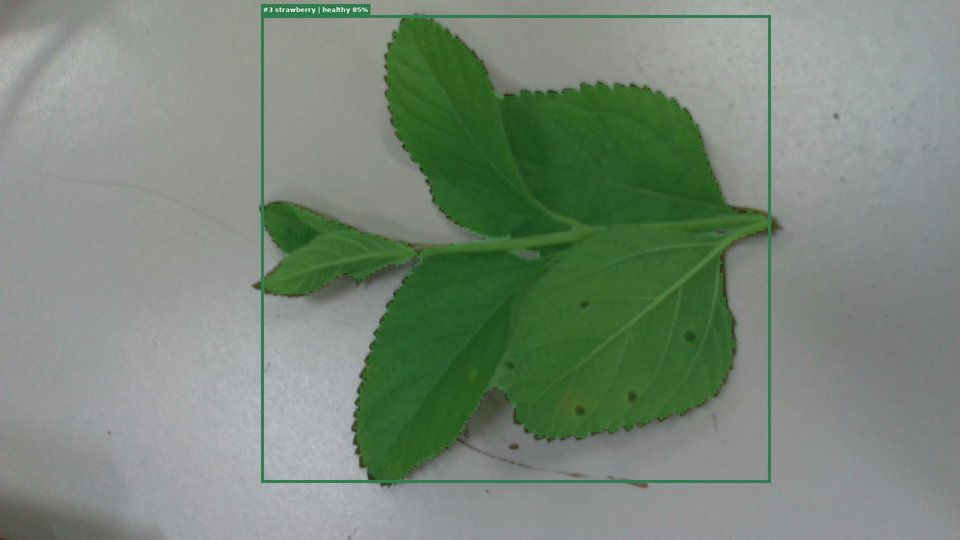
\includegraphics[width=\linewidth]{../figuras/bancada_saudavel.jpg}\\[2pt]
    \small \emph{healthy} 85\,\%
  \end{minipage}\hfill
  \begin{minipage}{0.325\linewidth}\centering
    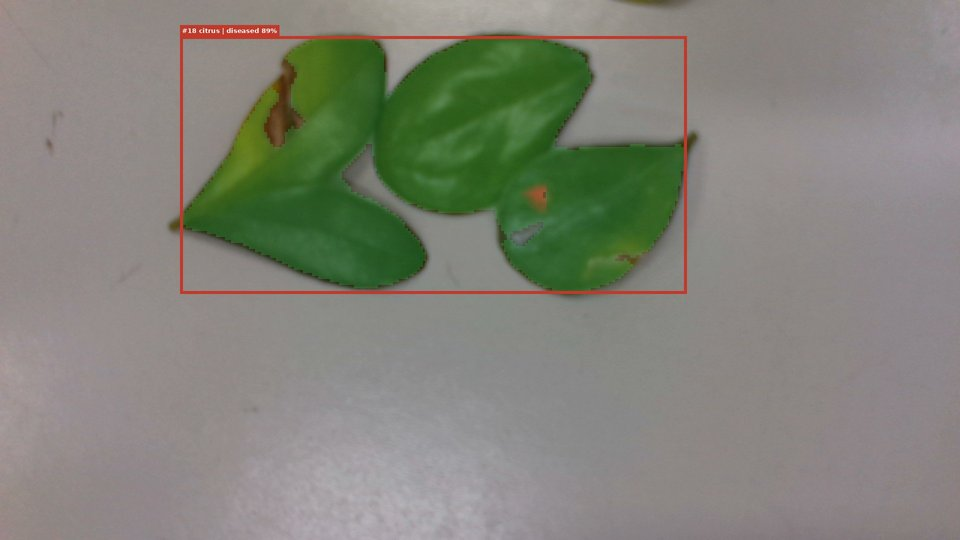
\includegraphics[width=\linewidth]{../figuras/bancada_doente.jpg}\\[2pt]
    \small \emph{diseased} 89\,\%, agente \emph{bacteria}
  \end{minipage}\hfill
  \begin{minipage}{0.325\linewidth}\centering
    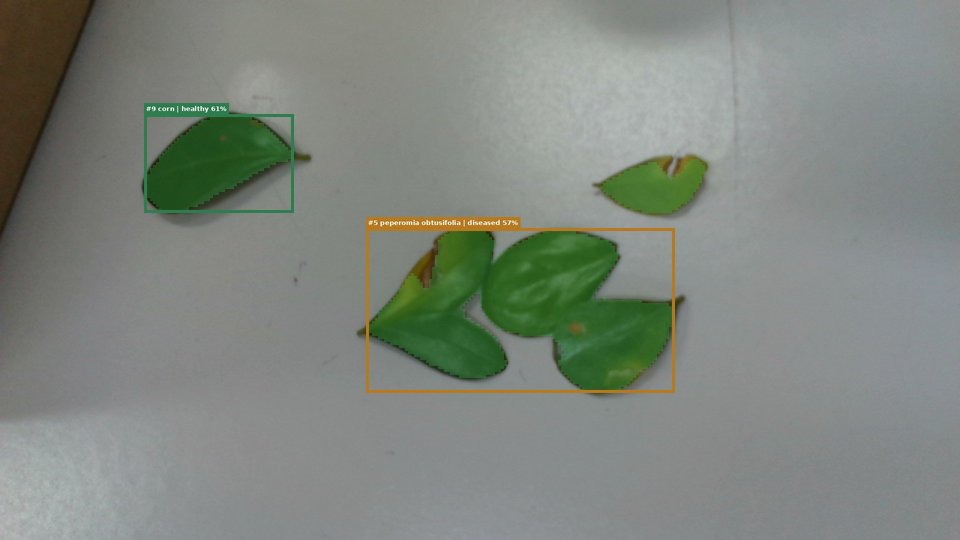
\includegraphics[width=\linewidth]{../figuras/bancada_mista.jpg}\\[2pt]
    \small \emph{healthy} 61\,\% e \emph{diseased} 57\,\%
  \end{minipage}
  \caption{Capturas reais da bancada com a RealSense D435, anotadas pelo servidor.}
  \label{fig:bancada}
\end{figure}

\begin{figure}[h]
  \centering
  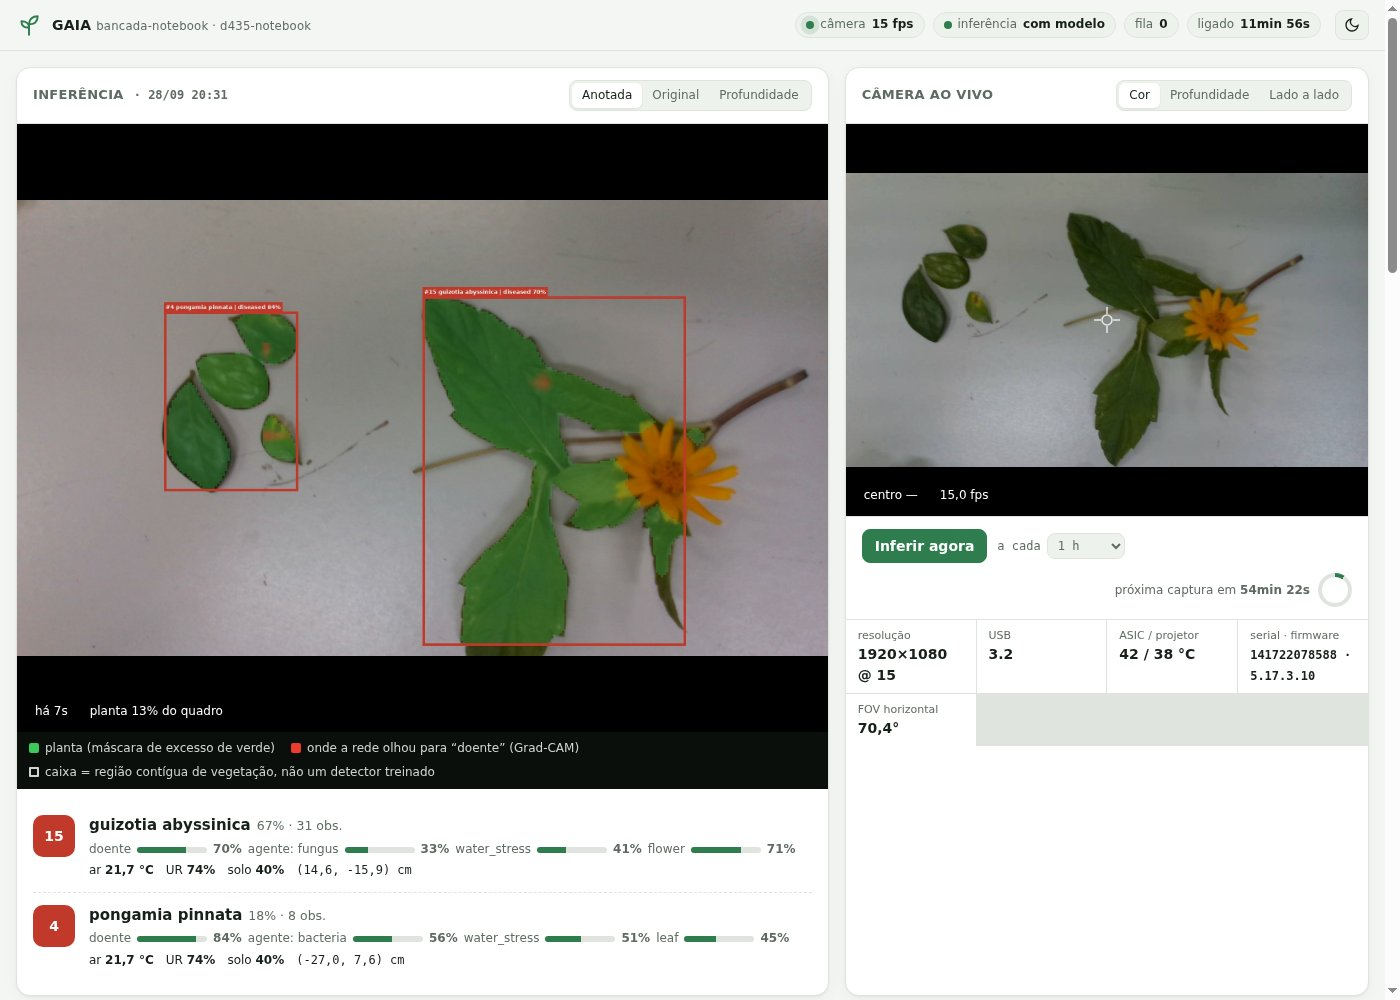
\includegraphics[width=0.92\linewidth]{../figuras/interface.jpg}
  \caption{Interface web do nó: a inferência como painel principal e a câmera ao vivo
  ao lado, com resolução, USB, temperatura do ASIC da câmera e o intervalo de captura.}
  \label{fig:interface}
\end{figure}

\begin{figure}[p]
  \centering
  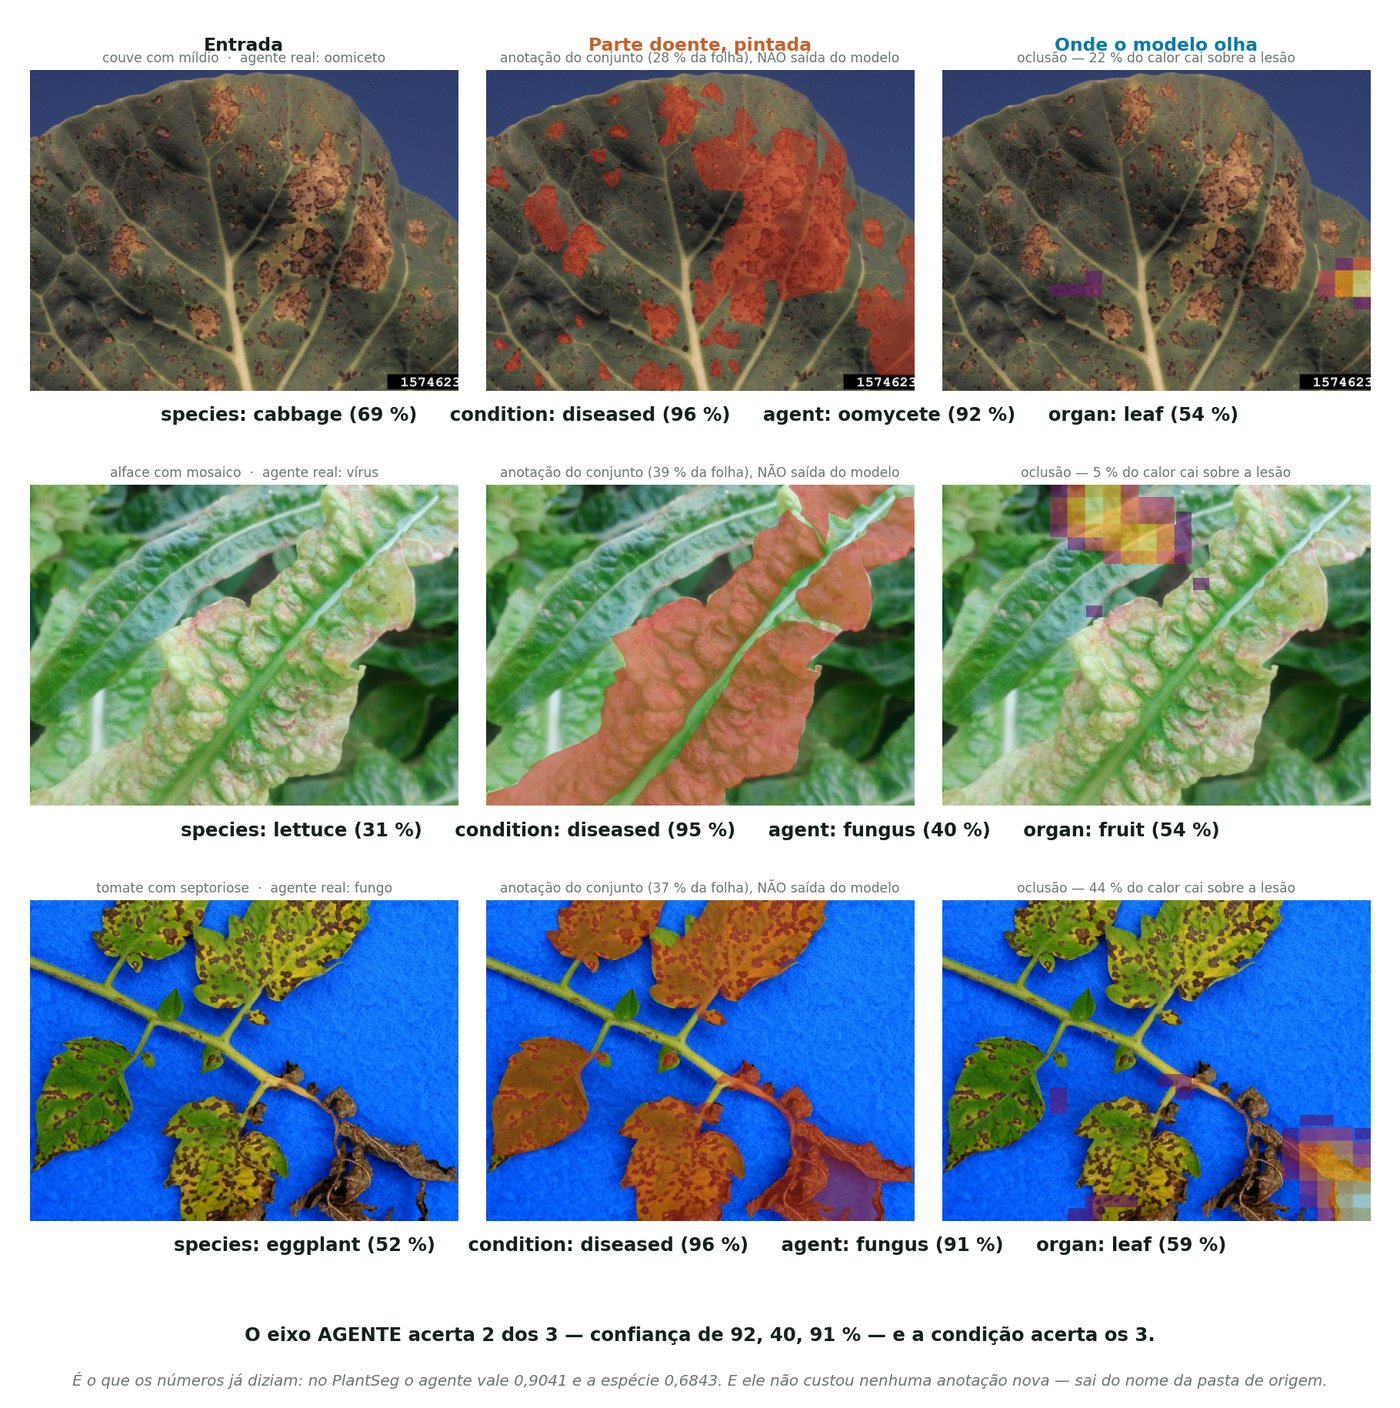
\includegraphics[width=0.82\linewidth]{../figuras/resultados_lesao.jpg}
  \caption{Resultado qualitativo do modelo: a entrada, a parte doente pintada, o mapa
  de oclusão e as cabeças com a confiança de cada uma.}
  \label{fig:lesao}
\end{figure}

\begin{figure}[h]
  \centering
  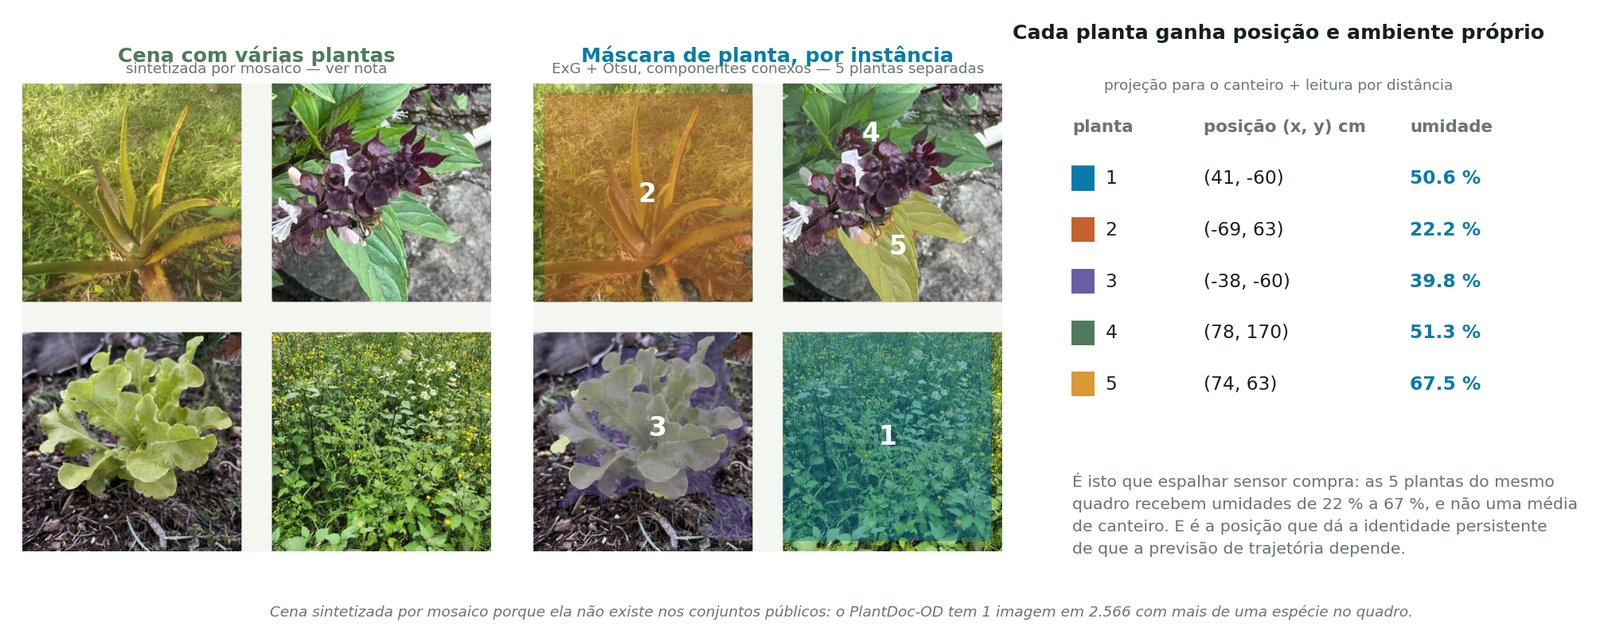
\includegraphics[width=\linewidth]{../figuras/resultados_cena.jpg}
  \caption{Cena com várias plantas: máscara por instância, projeção de cada planta
  para o canteiro e a umidade estimada no ponto de cada uma.}
  \label{fig:cena}
\end{figure}

\clearpage
% =====================================================================
\section{A rede}

Um modelo só, com um tronco compartilhado e uma cabeça por pergunta
(Figura~\ref{fig:rede}). Os sensores entram por um ramo à parte, somado às
features da imagem \textbf{apenas nas cabeças em que o ambiente importa}.

\begin{figure}[h]
\centering
\resizebox{\linewidth}{!}{%
\begin{tikzpicture}[
  >=Stealth, node distance=6mm and 9mm,
  caixa/.style={draw, rounded corners=3pt, align=center, font=\small,
                minimum height=10mm, inner sep=4pt, fill=white},
  tronco/.style={caixa, draw=black, line width=0.9pt, minimum width=36mm},
  sensor/.style={caixa, draw=azul, dashed, line width=0.8pt, text=azul},
  cabeca/.style={caixa, minimum width=24mm, minimum height=8mm},
  seta/.style={->, line width=0.7pt, draw=cinza}]

  \node[caixa, minimum width=34mm] (img) {Imagem RGB\\ \footnotesize Resize 1,14$\times$ + recorte 384$^2$};
  \node[tronco, right=of img] (tr) {Tronco ConvNeXt-Base\\ \footnotesize torchvision, 87,7\,M parâm.};
  \node[caixa, right=of tr, minimum width=20mm] (f) {features\\ 1024};

  \node[caixa, below=16mm of img, minimum width=34mm] (sen) {Sensores\\ \footnotesize temperatura, umidade do ar,\\ \footnotesize umidade do solo};
  \node[sensor, right=of sen, minimum width=36mm] (mlp) {Ramo de sensores\\ \footnotesize vetor 12 $\to$ 64 $\to$ 64 $\to$ 1024\\ \footnotesize última camada iniciada em zero};
  \node[sensor, right=of mlp, minimum width=20mm] (porta) {$\times$ porta\\ \footnotesize de presença};

  \node[circle, draw, line width=0.9pt, inner sep=1pt, font=\large] (soma) at ($(f.east)!0.5!(porta.east) + (14mm,0)$) {$+$};

  \node[cabeca, right=26mm of f, yshift=6mm] (sp) {\textbf{espécie} \footnotesize 1136};
  \node[cabeca, below=2mm of sp] (or) {\textbf{órgão} \footnotesize 6};
  \node[cabeca, right=12mm of soma, yshift=-1mm] (co) {\textbf{condição} \footnotesize 2};
  \node[cabeca, below=2mm of co] (ag) {\textbf{agente} \footnotesize 7};
  \node[cabeca, below=2mm of ag, draw=cinza, dashed, text=cinza] (hy) {\textbf{hidratação} \footnotesize 3};

  \draw[seta] (img) -- (tr);
  \draw[seta] (tr) -- (f);
  \draw[seta] (sen) -- (mlp);
  \draw[seta] (mlp) -- (porta);
  \draw[seta] (f.east) -- ++(4mm,0) |- (sp.west);
  \draw[seta] (f.east) -- ++(4mm,0) |- (or.west);
  \draw[seta] (f.south) |- (soma.west);
  \draw[seta] (porta.east) -| (soma.south);
  \draw[seta] (soma.east) -- ++(4mm,0) |- (co.west);
  \draw[seta] (soma.east) -- ++(4mm,0) |- (ag.west);
  \draw[seta] (soma.east) -- ++(4mm,0) |- (hy.west);
  \node[font=\footnotesize, text=laranja, right=2mm of co] {Grad-CAM};

  \begin{scope}[on background layer]
    \node[fill=fundo, rounded corners=4pt, fit=(sp)(or), inner sep=3mm,
          label={[font=\scriptsize, text=cinza]above:só imagem}] {};
    \node[fill=fundo, rounded corners=4pt, fit=(co)(ag)(hy), inner sep=3mm,
          label={[font=\scriptsize, text=cinza]below:imagem + sensores}] {};
  \end{scope}
\end{tikzpicture}}
\caption{A rede GAIA. Espécie e órgão usam as features puras da imagem; condição,
agente e hidratação usam imagem somada ao ramo de sensores. Tracejado: parte que
existe no modelo mas aguarda dado (o ramo de sensores e a cabeça de hidratação).}
\label{fig:rede}
\end{figure}

\begin{itemize}
  \item \textbf{Espécie e órgão} dependem só da aparência e usam as features puras.
  \item \textbf{Condição, agente e hidratação} usam imagem e sensores.
  \item O ramo de sensores nasce \textbf{neutro}: a projeção final começa em zero e a
  porta zera a contribuição quando não há leitura. O modelo é numericamente idêntico
  ao só-imagem até existir dado de sensor que ensine alguma coisa.
  \item Sensor ausente é ausente (flag~0), nunca zero.
\end{itemize}

\subsection{Entradas e saídas}
\paragraph{Imagem.} RGB, redimensionada para 1,14$\times$ o tamanho de entrada e
recortada no centro (384~px no ConvNeXt publicado). A borda da imagem não é vista
pela rede, e quem pinta explicação sobre a foto precisa levar isso em conta.

\paragraph{Sensores.} Temperatura (\textdegree C), umidade do ar (\%) e umidade do
solo (\%), todos opcionais. Viram um vetor de 12 posições: valor normalizado, flag de
presença, desvio da faixa ideal da espécie e flag do desvio.

\begin{table}[h]
\centering\small
\begin{tabularx}{0.92\linewidth}{@{}lX@{}}
\toprule
eixo & classes \\
\midrule
\cod{species}   & 1136 espécies \\
\cod{condition} & \emph{diseased}, \emph{healthy} \\
\cod{agent}     & \emph{none}, \emph{fungus}, \emph{oomycete}, \emph{bacteria}, \emph{virus}, \emph{pest}, \emph{abiotic} \\
\cod{organ}     & \emph{leaf}, \emph{flower}, \emph{fruit}, \emph{bark}, \emph{habit}, \emph{branch} \\
\cod{hydration} & \emph{hydrated}, \emph{water\_stress}, \emph{waterlogged} (ainda sem rótulo) \\
\bottomrule
\end{tabularx}
\caption{As cabeças de saída; cada uma tem softmax próprio.}
\end{table}

O checkpoint lista em \cod{trained\_axes} as cabeças que tiveram rótulo no treino.
As demais existem, mas a saída delas é ruído, e o preditor as marca como não
treinadas.

\subsection{Limites que as respostas não escondem}
\begin{itemize}
  \item \textbf{Espécie:} a confiança é baixa fora das fotos de laboratório (folha
  isolada, fundo limpo). No canteiro, a espécie é sugestão; a identidade da planta vem
  da posição.
  \item \textbf{Caixas:} saem da máscara de vegetação, não de um detector treinado.
  \item \textbf{Vermelho do Grad-CAM:} mostra onde a rede se apoiou para ``doente'',
  não mede lesão; o modelo nunca viu máscara de lesão no treino.
  \item \textbf{Ramo de sensores:} nenhuma imagem de treino tinha leitura de sensor.
  Até existir a série da horta, o efeito das leituras sobre a predição é pequeno.
\end{itemize}

% =====================================================================
\section{Etapa atual}

\newcommand{\estado}[2]{\item[#1] #2}
\begin{minipage}[t]{0.48\linewidth}
\textbf{Modelo}
\begin{itemize}[leftmargin=1.6em, labelsep=0.5em]
\estado{\feito}{Classificação multi-cabeça treinada (espécie, condição, agente, órgão)}
\estado{\feito}{Tronco ConvNeXt-Base a 384~px, robusto a borrão, baixa resolução e ruído}
\estado{\feito}{Ramo de sensores na arquitetura, neutro até haver dado}
\estado{\feito}{Explicação por Grad-CAM na cabeça de condição}
\estado{\falta}{Cabeça de hidratação com rótulo}
\estado{\falta}{Ramo de sensores treinado com leituras da horta}
\estado{\falta}{Cabeça de trajetória: ``não sustenta qualidade por mais $N$ dias''}
\estado{\falta}{Detector de plantas treinado}
\estado{\falta}{Modelo público (privado até o artigo)}
\end{itemize}
\end{minipage}\hfill
\begin{minipage}[t]{0.48\linewidth}
\textbf{Sistema}
\begin{itemize}[leftmargin=1.6em, labelsep=0.5em]
\estado{\feito}{Servidor com identidade por posição e sensores por distância}
\estado{\feito}{Nó com D435 (cor + profundidade), fila em disco e interface web}
\estado{\feito}{Sensores plugáveis}
\estado{\feito}{Inferência contínua na bancada, a cada 10~s}
\estado{\feito}{Imagem do SD com instalação offline, validada em ARM64 emulado}
\estado{\falta}{Validação no Raspberry Pi~3 físico}
\estado{\falta}{Coleta longitudinal na horta}
\estado{\falta}{Artigo}
\end{itemize}
\end{minipage}

\medskip
\noindent{\small\feito\ concluído \qquad \falta\ pendente}

% =====================================================================
\section{Servidor e inferência}

\subsection{Subir}
\begin{lstlisting}[language=bash]
pip install -r requirements.txt       # torch com CUDA: a versao da sua GPU
python3 servidor/baixar_modelo.py     # uma vez; modelo -> modelo/
cd servidor
./iniciar.sh                          # 0.0.0.0:8077, modelo de ../modelo
./iniciar.sh --com-simulada           # + uma estacao simulada em :8080
\end{lstlisting}

\begin{table}[h]
\centering\small
\begin{tabularx}{\linewidth}{@{}llX@{}}
\toprule
variável & padrão & para quê \\
\midrule
\cod{GAIA\_MODELO} & \cod{../modelo} & pasta ou \cod{.pt}; vazio = só ingestão, sem classificar \\
\cod{GAIA\_BANCO} & \cod{sqlite:///gaia.db} & qualquer URL do SQLAlchemy \\
\cod{GAIA\_MIDIA} & \cod{midia} & imagens, profundidade e anotações \\
\cod{GAIA\_REFERENCIA} & pasta do modelo & tabela de faixas ambientais por espécie \\
\bottomrule
\end{tabularx}
\end{table}

Sem modelo, o servidor funciona em \textbf{ingestão pura}: localiza plantas e guarda
a série e os sensores, o que permite começar a coletar antes de o modelo final
existir.

\subsection{Cadastro de canteiro, câmeras e sensores}
\begin{lstlisting}[language=bash]
python3 cadastrar.py local canteiro-1
python3 cadastrar.py camera d435-frontal --local 1 --x 0 --y -60 --z 80 --pitch -45 --fov 69.4
python3 cadastrar.py sensor ar --local 1 --canal temp --tipo temperature --central
python3 cadastrar.py sensor solo-a --local 1 --canal soil1 --tipo soil_moisture --x 20 --y 30
python3 cadastrar.py listar
\end{lstlisting}
\begin{itemize}
  \item Distâncias em cm a partir do controlador; ângulos em graus; \cod{pitch}
  negativo olha para baixo. A estação mostra o FOV exato, lido da câmera.
  \item \cod{--canal} é o nome que o nó envia. Canal não cadastrado é ignorado, então
  a temperatura da CPU pode ir junto sem poluir o dado da planta.
  \item \cod{--tipo} diz o que a leitura significa para o modelo. Só
  \cod{temperature}, \cod{air\_humidity} e \cod{soil\_moisture} entram no vetor de
  sensores.
  \item Bancada e canteiro real ficam em \textbf{locais diferentes}: dado de teste
  misturado à série de uma planta real não se separa depois.
\end{itemize}

\subsection{O pipeline do \texttt{/ingest}}
\begin{enumerate}
  \item \textbf{Plantas na imagem.} Máscara de vegetação pelo índice de excesso de
  verde (ExG) com limiar de Otsu e um piso absoluto de 0,10. Sem o piso, uma cena sem
  planta ainda teria ``metade verde''; medido com a D435, o teto branco chega a
  $p_{99} = 0{,}085$ e a folha passa de 0,5. Folhas próximas são agrupadas numa
  planta; cada grupo com mais de 1,5\,\% do quadro vira uma caixa (no máximo seis).
  Sem vegetação, não há caixa nem classificação.
  \item \textbf{Posição.} A base da caixa é projetada no plano do solo. Se o raio não
  cruza o solo, a detecção é guardada sem posição, em vez de inventar uma.
  \item \textbf{Identidade.} A planta mais próxima a menos de 20~cm, ou uma nova; a
  posição é refinada pela média a cada observação.
  \item \textbf{Sensores no ponto,} por inverso da distância; o sensor central é o
  fallback.
  \item \textbf{Classificação} do recorte com o vetor de sensores daquela planta.
  \item \textbf{Grad-CAM} da cabeça de condição no recorte, limitado à máscara de
  planta e com opacidade proporcional a $P(\text{doente})$.
  \item \textbf{Imagem anotada,} servida em \cod{/midia/...}.
\end{enumerate}

\subsection{API}
\begin{table}[h]
\centering\small
\begin{tabularx}{\linewidth}{@{}llX@{}}
\toprule
método & rota & o quê \\
\midrule
POST & \cod{/ingest} & multipart: \cod{imagem}, \cod{meta} (JSON), \cod{profundidade} (opcional) \\
GET & \cod{/saude} & estado do servidor e dos modelos \\
GET & \cod{/plantas} & plantas conhecidas, posição e número de observações \\
GET & \cod{/planta/\{id\}/serie} & série temporal de uma planta \\
GET & \cod{/midia/\{caminho\}} & imagens gravadas e anotadas \\
GET & \cod{/docs} & documentação interativa \\
\bottomrule
\end{tabularx}
\end{table}

\noindent O campo \cod{meta} do \cod{/ingest}:
\begin{lstlisting}
{
  "no": "canteiro-1",
  "camera": "d435-frontal",
  "instante": "2026-09-28T22:44:06+00:00",
  "imagem": "d435-frontal_20260928T224406Z.jpg",
  "leituras": {"temp": 24.1, "umid_ar": 66.0, "soil1": null},
  "camera_info": {"intrinseca_cor": {"fx": 615.3, "fy": 615.1, "cx": 322.5, "cy": 240.7}}
}
\end{lstlisting}
A câmera precisa estar cadastrada; sem extrínseca não há como projetar, e a resposta
é 404. Leitura \cod{null} significa ``sem leitura''. A resposta traz, por planta, a
posição, a espécie, a condição, o agente, a hidratação, o órgão (cada um com a
confiança), o ambiente estimado no ponto e a caixa, além do caminho da imagem anotada.

\subsection{Usar só a inferência}
\begin{lstlisting}[language=Python]
from gaia.preditor import Predictor
p = Predictor("modelo/")
r = p.predict("foto.jpg", readings={"temperature": 27.4, "air_humidity": 68})
print(r["condition"]["label"], r["condition"]["confidence"])
\end{lstlisting}

\subsection{Custo}
Numa RTX~3050 de 4~GB, o ConvNeXt a 384~px carrega em cerca de 4~s e classifica em
cerca de 0,35~s por recorte; o Grad-CAM custa uma passada para trás por recorte. Com
até seis plantas por quadro, um ciclo de 10~s cabe com folga. Nesse ritmo, as
imagens somam cerca de 700~MB por dia.

% =====================================================================
\section{Estação de captura e interface}

\begin{lstlisting}[language=bash]
cd estacao
python3 estacao.py --config estacao-notebook.json   # PC com a D435 no USB
python3 estacao.py --config estacao.json            # Pi (via systemd)
python3 estacao.py --simular                        # sem camera nem sensores
\end{lstlisting}
A estação usa só a biblioteca padrão do Python para o HTTP: num Pi de 1~GB cada
dependência pesa, e o FastAPI puxaria o \cod{pydantic-core}, que em armv7 compila em
Rust por horas. As dependências de fato são numpy, Pillow, requests e pyrealsense2.

\subsection{A interface}
\begin{itemize}
  \item \textbf{Inferência}, o painel principal: a última imagem, trocando sozinha a
  cada ciclo, com as abas anotada, original e profundidade, e abaixo cada planta com
  espécie, condição, agente, hidratação, órgão e o ambiente no ponto.
  \item \textbf{Câmera ao vivo}: MJPEG de cor, profundidade ou lado a lado; distância
  no centro; temperatura do ASIC; botão ``Inferir agora'' e intervalo de 5~s a 1~h.
  \item \textbf{Sensores}, \textbf{histórico} (1~h a 7~dias), \textbf{capturas} e
  \textbf{sistema}.
\end{itemize}
A página é um único arquivo, sem CDN, porque o Pi pode estar sem internet.

\subsection{Configuração}
O campo \cod{servidor} é uma lista: vale o primeiro que responder \cod{/saude}, de
modo que o mesmo arquivo serve no cabo, no hotspot e na VM. O modo \cod{--simular}
troca a câmera por uma cena sintética e cada sensor de hardware por um simulado nos
mesmos canais, gravando como outra câmera, numa pasta à parte.

\subsection{Sensores plugáveis}
\begin{table}[h]
\centering\small
\begin{tabularx}{\linewidth}{@{}lX@{}}
\toprule
tipo & observação \\
\midrule
\cod{cpu} & temperatura do SoC \\
\cod{realsense} & ASIC e projetor da D435; acusa câmera cozinhando ao sol \\
\cod{dht11}, \cod{dht22} & temperatura e umidade do ar num GPIO digital \\
\cod{ds18b20} & 1-Wire, lido pelo sysfs \\
\cod{mcp3008} & umidade do solo por ADC SPI (o Pi não tem entrada analógica) \\
\cod{comando} & qualquer programa que imprima um número \\
\cod{simulado} & ciclo diário com ruído e falhas ocasionais \\
\bottomrule
\end{tabularx}
\end{table}

\subsection{RealSense D435}
Um pipeline só: uma thread guarda o último quadro para o vídeo ao vivo, e a captura
pede o próximo quadro \textbf{alinhado}, com a profundidade reprojetada na geometria
da cor. No PC, a cor vai a 1920$\times$1080 e a profundidade a 1280$\times$720; em
USB~2, caso do Pi~3, a estação força 640$\times$480 a 15~fps. A captura guarda a
intrínseca de fábrica, o que abre caminho para a projeção sem trena, e a profundidade
por pixel, a primeira medida métrica da planta.

% =====================================================================
\section{Raspberry Pi}

\subsection{Sistema e instalação offline}
O \cod{pyrealsense2} só publica wheel aarch64 para Python 3.8 e 3.9, então o sistema
é o Raspberry Pi OS Lite 64-bit \emph{bullseye} (Python 3.9). O bullseye saiu de
suporte em 2026-08, e o repositório de segurança já anuncia pacotes removidos. Por
isso a instalação é \textbf{100\,\% offline}: no PC, \cod{montar\_offline.sh} baixa
numpy, Pillow, pyrealsense2, requests e a pilha do DHT como wheels aarch64, além da
\cod{libusb} de que o pyrealsense2 precisa; no Pi, \cod{instalar\_pi.sh} os extrai
sem \cod{apt}, \cod{venv} nem \cod{pip}.

\begin{lstlisting}[language=bash]
cd estacao/imagem
./montar_offline.sh
GAIA_ETH_IP=192.168.123.144/24 GAIA_ETH_GW=192.168.123.99 ./gerar_imagem.sh
lsblk -o NAME,SIZE,MODEL,TRAN               # confira o dispositivo
sudo dd if=gaia-pi.img of=/dev/sdX bs=4M conv=fsync status=progress
\end{lstlisting}

No primeiro boot, a imagem expande a partição, configura hostname, usuário, SSH e
rede, copia o código e instala a estação sozinha. O IP pode ser trocado sem regravar
o cartão, editando \cod{gaia-rede.conf} na partição de boot.

\subsection{Rede}
O caminho mais simples é o \textbf{cabo direto no PC}: o PC vira 192.168.123.99 e
compartilha a internet do Wi-Fi dele (\cod{servidor/cabo.sh}). O DNS padrão do Pi é o
próprio gateway, porque redes de laboratório costumam bloquear servidores públicos
como 1.1.1.1 e 8.8.8.8. Também há um hotspot em 2,4~GHz (\cod{servidor/hotspot.sh}).

\subsection{Sem tela nem teclado}
\begin{itemize}
  \item \cod{servidor/achar\_pi.sh -f} varre a rede e diz a etapa: fora da rede,
  instalando (só SSH) ou interface no ar. Ignora celulares pelo endereço MAC.
  \item Pelo SSH: \cod{journalctl -fu gaia-instalar} e \cod{systemctl status gaia-estacao}.
  \item Sem acesso nenhum: tirar o cartão e ler, no PC, os logs \cod{gaia-firstrun.log},
  \cod{gaia-instalacao.log} e \cod{gaia-rede.log} da partição de boot.
\end{itemize}

\subsection{Ligação do DHT11}
\begin{table}[h]
\centering\small
\begin{tabular}{@{}lll@{}}
\toprule
DHT11 & Raspberry Pi 3 B/B+ & observação \\
\midrule
VCC (+) & pino 1 --- 3,3\,V & \textbf{não} usar 5\,V: o GPIO só aguenta 3,3\,V \\
DATA & pino 7 --- GPIO4 & 10\,k$\Omega$ entre DATA e VCC no sensor de 4 pinos \\
GND ($-$) & pino 6 --- GND & \\
\bottomrule
\end{tabular}
\end{table}
O módulo de três pinos numa plaquinha já tem o resistor de pull-up. A D435 no Pi~3
puxa até cerca de 700~mA: use fonte de 2,5~A e, de preferência, um hub USB
alimentado.

\subsection{Testar sem hardware}
Uma VM QEMU (máquina \cod{virt}, Cortex-A53, 4~núcleos, 1~GB) reproduz o orçamento do
Pi~3 e aceita a D435 pelo xHCI. Para validar só a instalação offline, basta um
container \cod{arm64v8/python:3.9-slim-bullseye} com \cod{--network none}; foi assim
que se descobriu a dependência da \cod{libusb}.

% =====================================================================
\section{Criando outros protótipos}

O contrato entre as partes é pequeno: o nó envia \cod{POST /ingest} com uma imagem e
um JSON de leituras por canal, e o servidor sabe onde cada câmera e cada sensor
estão.

\paragraph{Um sensor novo.} Sem código, pelo tipo \cod{comando}; com código, uma
classe em \cod{estacao/sensores.py}:
\begin{lstlisting}[language=Python]
class BH1750(Driver):
    def descrever(self):
        return [(self.cfg.get("canal", "luz"), "Luminosidade", "lx")]

    def ler(self):
        try:
            return {self.descrever()[0][0]: ler_bh1750(self.cfg.get("endereco", 0x23))}
        except Exception:
            return {self.descrever()[0][0]: None}   # falha = None

TIPOS["bh1750"] = BH1750
\end{lstlisting}
Para o modelo usar a leitura, ela precisa ser de um tipo que ele conhece; um tipo
novo exige retreinar o ramo de sensores.

\paragraph{Um nó em outro hardware.} Qualquer dispositivo capaz de um POST multipart
é um nó (ESP32-CAM, celular, outro computador de placa única). Regras que valem para
todos:
\begin{enumerate}
  \item cadastrar a câmera no servidor, com posição, ângulos, FOV e resolução;
  \item gravar antes de enviar;
  \item manter o relógio certo, porque o instante vem do nó e um Pi sem RTC acorda com
  a data da última vez que desligou;
  \item enviar \cod{null} para ``sem leitura'': zero é leitura.
\end{enumerate}

\paragraph{Mais de uma câmera.} Cada uma com a própria posição. Como a identidade é
pela coordenada no canteiro, a mesma planta vista por duas câmeras cai no mesmo
identificador.

\paragraph{Outra forma de achar plantas.} Um detector treinado entra implementando a
mesma assinatura de \cod{caixas\_pela\_mascara}, que devolve a máscara e as caixas.

\paragraph{Outro modelo.} O preditor lê do checkpoint a arquitetura, o tamanho de
entrada, as classes e o ramo de sensores. Qualquer checkpoint no mesmo formato
funciona sem mudar código; uma MobileNet roda em CPU e serve para servidor sem GPU.

% =====================================================================
\section{Publicação do modelo}
O modelo não está no repositório de código. Ele é exportado só com o que a inferência
usa e publicado no Hugging Face:
\begin{lstlisting}[language=bash]
python3 ferramentas/exportar_modelo.py best.pt publicar/ species_env.csv
huggingface-cli upload <usuario>/<repositorio> publicar/ . --repo-type model
python3 servidor/baixar_modelo.py --repo <usuario>/<repositorio>
\end{lstlisting}
São publicados os pesos com a configuração e as classes, a lista de classes em JSON,
a tabela de faixas ambientais por espécie e o cartão do modelo. O arquivo \cod{.pt} é
um pickle do PyTorch: carregue apenas checkpoints de fonte confiável.

% =====================================================================
\section*{Referências}
\addcontentsline{toc}{section}{Referências}
\small
\begin{description}[style=nextline, leftmargin=0pt, font=\normalfont\bfseries]
\item[Modelo e métodos]
Z.~Liu, H.~Mao, C.-Y.~Wu, C.~Feichtenhofer, T.~Darrell, S.~Xie. \emph{A ConvNet for
the 2020s.} CVPR, 2022.\\
R.~R.~Selvaraju, M.~Cogswell, A.~Das, R.~Vedantam, D.~Parikh, D.~Batra.
\emph{Grad-CAM: Visual Explanations from Deep Networks via Gradient-based
Localization.} ICCV, 2017.\\
D.~M.~Woebbecke, G.~E.~Meyer, K.~Von~Bargen, D.~A.~Mortensen. \emph{Color indices
for weed identification under various soil, residue, and lighting conditions.}
Transactions of the ASAE, 38(1), 1995.\\
N.~Otsu. \emph{A threshold selection method from gray-level histograms.} IEEE
Transactions on Systems, Man, and Cybernetics, 9(1), 1979.
\item[Conjuntos de dados usados no treino (não distribuídos)]
D.~P.~Hughes, M.~Salathé. \emph{An open access repository of images on plant health
to enable the development of mobile disease diagnostics.} arXiv:1511.08060, 2015
(PlantVillage).\\
D.~Singh, N.~Jain, P.~Jain, P.~Kayal, S.~Kumawat, N.~Batra. \emph{PlantDoc: A Dataset
for Visual Plant Disease Detection.} CoDS-COMAD, 2020.\\
C.~Garcin et al. \emph{Pl@ntNet-300K: a plant image dataset with high label ambiguity
and a long-tailed distribution.} NeurIPS Datasets and Benchmarks, 2021.\\
T.~Wei et al. \emph{PlantSeg: A Large-Scale In-the-wild Dataset for Plant Disease
Segmentation.} arXiv:2409.04038, 2024.\\
GBIF.org --- Global Biodiversity Information Facility, ocorrências com imagem.
\item[Hardware e software]
Intel RealSense D400 Series Product Family Datasheet; librealsense e pyrealsense2.
PyTorch e torchvision; FastAPI; SQLAlchemy; Raspberry Pi OS.
\end{description}

\end{document}
